\documentclass[11pt,a4paper]{article}
\usepackage[T1]{fontenc}
\usepackage[utf8]{inputenc}
\usepackage{lmodern}
\usepackage[margin=2.5cm]{geometry}
\usepackage{amsmath}
\usepackage{graphicx}
\usepackage{booktabs}
\usepackage{array}
\usepackage[section]{placeins}
\usepackage{caption}
\usepackage{enumitem}
\usepackage{xr-hyper}
\usepackage[hidelinks]{hyperref}
\usepackage{xurl}
\externaldocument[M-]{../paper/paper}
\captionsetup{font=small,labelfont=bf}
\setlist{itemsep=2pt,topsep=4pt}
\expandafter\def\csname res@Tc\endcsname{3272}
\expandafter\def\csname res@altApForty\endcsname{227}
\expandafter\def\csname res@altApTwenty\endcsname{190}
\expandafter\def\csname res@altGainHigh\endcsname{1.3}
\expandafter\def\csname res@altGainLow\endcsname{2.4}
\expandafter\def\csname res@altVForty\endcsname{240\,000}
\expandafter\def\csname res@altVTwenty\endcsname{4\,500}
\expandafter\def\csname res@altVolRatioHigh\endcsname{8.9}
\expandafter\def\csname res@altVolRatioLow\endcsname{6.0}
\expandafter\def\csname res@atmP\endcsname{1197}
\expandafter\def\csname res@atmRho\endcsname{0.0184}
\expandafter\def\csname res@atmT\endcsname{226.5}
\expandafter\def\csname res@audDiv\endcsname{60.45}
\expandafter\def\csname res@audDvBack\endcsname{2173}
\expandafter\def\csname res@audDvPct\endcsname{24}
\expandafter\def\csname res@audEratio\endcsname{34}
\expandafter\def\csname res@audGasRatio\endcsname{11.5}
\expandafter\def\csname res@audH2ratio\endcsname{70}
\expandafter\def\csname res@audLnA\endcsname{0.916}
\expandafter\def\csname res@audLnB\endcsname{1.253}
\expandafter\def\csname res@audMolar\endcsname{947}
\expandafter\def\csname res@audPratio\endcsname{9.8}
\expandafter\def\csname res@audRhoLow\endcsname{1.8}
\expandafter\def\csname res@audRhoRatio\endcsname{10.4}
\expandafter\def\csname res@audRhoTot\endcsname{56}
\expandafter\def\csname res@audVolRatio\endcsname{6.1}
\expandafter\def\csname res@balAp\endcsname{214}
\expandafter\def\csname res@balArea\endcsname{4347}
\expandafter\def\csname res@balBareH2\endcsname{22.5}
\expandafter\def\csname res@balBareV\endcsname{17\,600}
\expandafter\def\csname res@balDv\endcsname{2091}
\expandafter\def\csname res@balEnv\endcsname{130}
\expandafter\def\csname res@balEps\endcsname{36.4}
\expandafter\def\csname res@balF\endcsname{11.8}
\expandafter\def\csname res@balH2\endcsname{34.5}
\expandafter\def\csname res@balHb\endcsname{58.0}
\expandafter\def\csname res@balHe\endcsname{75.4}
\expandafter\def\csname res@balHeMassRatio\endcsname{2.18}
\expandafter\def\csname res@balHeVolPct\endcsname{10}
\expandafter\def\csname res@balIsp\endcsname{303.4}
\expandafter\def\csname res@balIspVac\endcsname{307.3}
\expandafter\def\csname res@balLaunchH2\endcsname{38}
\expandafter\def\csname res@balLd\endcsname{8}
\expandafter\def\csname res@balLg\endcsname{369}
\expandafter\def\csname res@balMdot\endcsname{3.97}
\expandafter\def\csname res@balPe\endcsname{4.7}
\expandafter\def\csname res@balQ\endcsname{1.7}
\expandafter\def\csname res@balTap\endcsname{222}
\expandafter\def\csname res@balTb\endcsname{38.1}
\expandafter\def\csname res@balV\endcsname{27\,000}
\expandafter\def\csname res@balVHe\endcsname{29\,600}
\expandafter\def\csname res@balVHi\endcsname{30\,300}
\expandafter\def\csname res@balVLo\endcsname{24\,000}
\expandafter\def\csname res@balVb\endcsname{1714}
\expandafter\def\csname res@betaBase\endcsname{2397}
\expandafter\def\csname res@betaHi\endcsname{4506}
\expandafter\def\csname res@betaLo\endcsname{1046}
\expandafter\def\csname res@bmCstar\endcsname{1726}
\expandafter\def\csname res@bmFrozen\endcsname{274.9}
\expandafter\def\csname res@bmShift\endcsname{285.9}
\expandafter\def\csname res@bmTc\endcsname{3426}
\expandafter\def\csname res@cBalD\endcsname{0.31}
\expandafter\def\csname res@cBalDry\endcsname{90.4}
\expandafter\def\csname res@cBalEnv\endcsname{89}
\expandafter\def\csname res@cBalF\endcsname{5.5}
\expandafter\def\csname res@cBalGas\endcsname{19.3}
\expandafter\def\csname res@cBalM\endcsname{140}
\expandafter\def\csname res@cBalMSS\endcsname{168}
\expandafter\def\csname res@cBalMp\endcsname{49.6}
\expandafter\def\csname res@cBalTb\endcsname{27.1}
\expandafter\def\csname res@cBalV\endcsname{15\,100}
\expandafter\def\csname res@cGndM\endcsname{348}
\expandafter\def\csname res@cGndMSS\endcsname{755}
\expandafter\def\csname res@cGndMp\endcsname{222}
\expandafter\def\csname res@cMassRatio\endcsname{2.5}
\expandafter\def\csname res@cPropRatio\endcsname{4.5}
\expandafter\def\csname res@cSysBal\endcsname{280}
\expandafter\def\csname res@cTwentyM\endcsname{152}
\expandafter\def\csname res@cTwentyV\endcsname{2\,500}
\expandafter\def\csname res@cstar\endcsname{1720}
\expandafter\def\csname res@deaCdFit\endcsname{1.16}
\expandafter\def\csname res@deaD\endcsname{0.171}
\expandafter\def\csname res@deaDragShare\endcsname{8}
\expandafter\def\csname res@deaErrCold\endcsname{+6.2}
\expandafter\def\csname res@deaErrMaxAbs\endcsname{2.6}
\expandafter\def\csname res@deaErrMean\endcsname{+1.3}
\expandafter\def\csname res@deaGroundHeavy\endcsname{22}
\expandafter\def\csname res@deaGroundLight\endcsname{25}
\expandafter\def\csname res@deaImp\endcsname{87.5}
\expandafter\def\csname res@deaIsp\endcsname{191}
\expandafter\def\csname res@deaMp\endcsname{46.7}
\expandafter\def\csname res@deaRmsFit\endcsname{0.8}
\expandafter\def\csname res@deaRmsUnit\endcsname{1.4}
\expandafter\def\csname res@decAltTenBal\endcsname{127}
\expandafter\def\csname res@decAltTenDrag\endcsname{63}
\expandafter\def\csname res@decAltTenGnd\endcsname{35}
\expandafter\def\csname res@decAltTenHead\endcsname{11}
\expandafter\def\csname res@decAltTenNozzle\endcsname{26}
\expandafter\def\csname res@decAltTenRatio\endcsname{3.7}
\expandafter\def\csname res@decAltTwentyBal\endcsname{190}
\expandafter\def\csname res@decAltTwentyDrag\endcsname{56}
\expandafter\def\csname res@decAltTwentyGnd\endcsname{35}
\expandafter\def\csname res@decAltTwentyHead\endcsname{13}
\expandafter\def\csname res@decAltTwentyNozzle\endcsname{31}
\expandafter\def\csname res@decAltTwentyRatio\endcsname{5.5}
\expandafter\def\csname res@decDrag\endcsname{93}
\expandafter\def\csname res@decFDrag\endcsname{52}
\expandafter\def\csname res@decFHead\endcsname{17}
\expandafter\def\csname res@decFNozzle\endcsname{31}
\expandafter\def\csname res@decHead\endcsname{31}
\expandafter\def\csname res@decMassBigBal\endcsname{203}
\expandafter\def\csname res@decMassBigDrag\endcsname{41}
\expandafter\def\csname res@decMassBigGnd\endcsname{60}
\expandafter\def\csname res@decMassBigHead\endcsname{22}
\expandafter\def\csname res@decMassBigNozzle\endcsname{37}
\expandafter\def\csname res@decMassBigRatio\endcsname{3.4}
\expandafter\def\csname res@decMassFiftyBal\endcsname{221}
\expandafter\def\csname res@decMassFiftyDrag\endcsname{60}
\expandafter\def\csname res@decMassFiftyGnd\endcsname{18}
\expandafter\def\csname res@decMassFiftyHead\endcsname{15}
\expandafter\def\csname res@decMassFiftyNozzle\endcsname{24}
\expandafter\def\csname res@decMassFiftyRatio\endcsname{12.4}
\expandafter\def\csname res@decNozzle\endcsname{56}
\expandafter\def\csname res@dryFor100\endcsname{269}
\expandafter\def\csname res@dvCap\endcsname{991}
\expandafter\def\csname res@dvCapOpt\endcsname{1235}
\expandafter\def\csname res@fallAp\endcsname{181}
\expandafter\def\csname res@fallCost\endcsname{33}
\expandafter\def\csname res@fallDv\endcsname{2086}
\expandafter\def\csname res@fallEps\endcsname{36.4}
\expandafter\def\csname res@fallF\endcsname{11.8}
\expandafter\def\csname res@fallHb\endcsname{51.5}
\expandafter\def\csname res@fallIsp\endcsname{302.8}
\expandafter\def\csname res@fallIspVac\endcsname{307.3}
\expandafter\def\csname res@fallLd\endcsname{10}
\expandafter\def\csname res@fallLg\endcsname{369}
\expandafter\def\csname res@fallMdot\endcsname{3.98}
\expandafter\def\csname res@fallPe\endcsname{4.7}
\expandafter\def\csname res@fallQ\endcsname{2.2}
\expandafter\def\csname res@fallSpeed\endcsname{139}
\expandafter\def\csname res@fallTap\endcsname{205}
\expandafter\def\csname res@fallTb\endcsname{38.0}
\expandafter\def\csname res@fallVb\endcsname{1567}
\expandafter\def\csname res@feedAl\endcsname{0.211}
\expandafter\def\csname res@feedSS\endcsname{0.477}
\expandafter\def\csname res@filmAreal\endcsname{18.4}
\expandafter\def\csname res@frDeficitPct\endcsname{15}
\expandafter\def\csname res@frDel\endcsname{246}
\expandafter\def\csname res@frFrozen\endcsname{241.4}
\expandafter\def\csname res@frShift\endcsname{267.9}
\expandafter\def\csname res@frTc\endcsname{1443}
\expandafter\def\csname res@ftAl\endcsname{0.060}
\expandafter\def\csname res@ftHP\endcsname{1.97}
\expandafter\def\csname res@ftSS\endcsname{0.237}
\expandafter\def\csname res@gainKm\endcsname{179}
\expandafter\def\csname res@gainRatio\endcsname{6.2}
\expandafter\def\csname res@gasH2\endcsname{0.0748}
\expandafter\def\csname res@gasHe\endcsname{0.160}
\expandafter\def\csname res@gndAp\endcsname{35}
\expandafter\def\csname res@gndDv\endcsname{1636}
\expandafter\def\csname res@gndEps\endcsname{3.68}
\expandafter\def\csname res@gndF\endcsname{11.8}
\expandafter\def\csname res@gndFirstTen\endcsname{9.2}
\expandafter\def\csname res@gndHb\endcsname{11.7}
\expandafter\def\csname res@gndIsp\endcsname{226.4}
\expandafter\def\csname res@gndIspVac\endcsname{259.0}
\expandafter\def\csname res@gndLd\endcsname{508}
\expandafter\def\csname res@gndLg\endcsname{278}
\expandafter\def\csname res@gndMdot\endcsname{5.32}
\expandafter\def\csname res@gndPe\endcsname{106.0}
\expandafter\def\csname res@gndQ\endcsname{121}
\expandafter\def\csname res@gndTap\endcsname{95}
\expandafter\def\csname res@gndTb\endcsname{28.4}
\expandafter\def\csname res@gndVb\endcsname{850}
\expandafter\def\csname res@h2oRatio\endcsname{6}
\expandafter\def\csname res@heBottleHi\endcsname{2.6}
\expandafter\def\csname res@heBottleKg\endcsname{0.113}
\expandafter\def\csname res@heBottleLo\endcsname{1.4}
\expandafter\def\csname res@heBottleMid\endcsname{1.8}
\expandafter\def\csname res@heKg\endcsname{0.0085}
\expandafter\def\csname res@heMassHi\endcsname{50}
\expandafter\def\csname res@heMassLo\endcsname{26}
\expandafter\def\csname res@heMassMid\endcsname{34}
\expandafter\def\csname res@heVolHi\endcsname{872}
\expandafter\def\csname res@heVolLo\endcsname{453}
\expandafter\def\csname res@heVolMid\endcsname{597}
\expandafter\def\csname res@ispDel\endcsname{307.3}
\expandafter\def\csname res@ispDelHi\endcsname{317}
\expandafter\def\csname res@ispDelLo\endcsname{284}
\expandafter\def\csname res@ispFrozen\endcsname{312.9}
\expandafter\def\csname res@ispFrozenPeak\endcsname{315.0}
\expandafter\def\csname res@ispShift\endcsname{334.0}
\expandafter\def\csname res@ispShiftPeak\endcsname{335.8}
\expandafter\def\csname res@lapP\endcsname{270}
\expandafter\def\csname res@lapRho\endcsname{0.0101}
\expandafter\def\csname res@lapT\endcsname{93.45}
\expandafter\def\csname res@lapZero\endcsname{44}
\expandafter\def\csname res@mapApTen\endcsname{127}
\expandafter\def\csname res@mcBalCv\endcsname{9}
\expandafter\def\csname res@mcBalHi\endcsname{238}
\expandafter\def\csname res@mcBalLo\endcsname{176}
\expandafter\def\csname res@mcBalMed\endcsname{204}
\expandafter\def\csname res@mcDragLargest\endcsname{100}
\expandafter\def\csname res@mcFDragHi\endcsname{56}
\expandafter\def\csname res@mcFDragLo\endcsname{46}
\expandafter\def\csname res@mcFDragMed\endcsname{51}
\expandafter\def\csname res@mcFHeadHi\endcsname{21}
\expandafter\def\csname res@mcFHeadLo\endcsname{16}
\expandafter\def\csname res@mcFHeadMed\endcsname{18}
\expandafter\def\csname res@mcFNozzleHi\endcsname{34}
\expandafter\def\csname res@mcFNozzleLo\endcsname{27}
\expandafter\def\csname res@mcFNozzleMed\endcsname{30}
\expandafter\def\csname res@mcGndCv\endcsname{18}
\expandafter\def\csname res@mcGndHi\endcsname{43}
\expandafter\def\csname res@mcGndLo\endcsname{24}
\expandafter\def\csname res@mcGndMed\endcsname{32}
\expandafter\def\csname res@mcN\endcsname{10\,000}
\expandafter\def\csname res@mcNshap\endcsname{1\,000}
\expandafter\def\csname res@mcPbelow\endcsname{0.0}
\expandafter\def\csname res@mcRatioHi\endcsname{8.0}
\expandafter\def\csname res@mcRatioLo\endcsname{5.0}
\expandafter\def\csname res@mcRatioMed\endcsname{6.3}
\expandafter\def\csname res@mpFor100\endcsname{82}
\expandafter\def\csname res@mrCap\endcsname{1.51}
\expandafter\def\csname res@nacaMassHi\endcsname{106}
\expandafter\def\csname res@nacaMassLo\endcsname{86}
\expandafter\def\csname res@ofFrozenPeak\endcsname{2.05}
\expandafter\def\csname res@ofShiftPeak\endcsname{2.75}
\expandafter\def\csname res@peakAccel\endcsname{8.1}
\expandafter\def\csname res@propFrac\endcsname{0.502}
\expandafter\def\csname res@propH2Ratio\endcsname{7.5}
\expandafter\def\csname res@propRhoOwn\endcsname{0.099}
\expandafter\def\csname res@propVolL\endcsname{156}
\expandafter\def\csname res@propVolRatio\endcsname{9.4}
\expandafter\def\csname res@rhoBalCd\endcsname{-0.02}
\expandafter\def\csname res@rhoBalDry\endcsname{-0.70}
\expandafter\def\csname res@rhoBalEta\endcsname{+0.66}
\expandafter\def\csname res@rhoBalTw\endcsname{+0.20}
\expandafter\def\csname res@rhoBalZf\endcsname{+0.10}
\expandafter\def\csname res@rhoGndCd\endcsname{-0.70}
\expandafter\def\csname res@rhoGndDry\endcsname{-0.31}
\expandafter\def\csname res@rhoGndEta\endcsname{+0.58}
\expandafter\def\csname res@rhoGndTw\endcsname{-0.23}
\expandafter\def\csname res@rhoGndZf\endcsname{-0.01}
\expandafter\def\csname res@rhoH2float\endcsname{0.00128}
\expandafter\def\csname res@runBBB\endcsname{214}
\expandafter\def\csname res@runBBG\endcsname{144}
\expandafter\def\csname res@runBGB\endcsname{106}
\expandafter\def\csname res@runBGG\endcsname{65}
\expandafter\def\csname res@runGBB\endcsname{182}
\expandafter\def\csname res@runGBG\endcsname{112}
\expandafter\def\csname res@runGGB\endcsname{75}
\expandafter\def\csname res@runGGG\endcsname{35}
\expandafter\def\csname res@sCdHi\endcsname{212}
\expandafter\def\csname res@sCdLo\endcsname{215}
\expandafter\def\csname res@sEtaHi\endcsname{227}
\expandafter\def\csname res@sEtaLo\endcsname{185}
\expandafter\def\csname res@sGndCdHi\endcsname{28}
\expandafter\def\csname res@sGndCdLo\endcsname{43}
\expandafter\def\csname res@sGndD30\endcsname{58}
\expandafter\def\csname res@sGndD35\endcsname{45}
\expandafter\def\csname res@sTwHi\endcsname{221}
\expandafter\def\csname res@sTwLo\endcsname{176}
\expandafter\def\csname res@suiApHeavy\endcsname{60}
\expandafter\def\csname res@suiApLight\endcsname{91}
\expandafter\def\csname res@suiFire\endcsname{11.6}
\expandafter\def\csname res@suiMassFit\endcsname{103}
\expandafter\def\csname res@suiMassHi\endcsname{103}
\expandafter\def\csname res@suiMassLo\endcsname{107}
\expandafter\def\csname res@suiMassMid\endcsname{105}
\expandafter\def\csname res@suiTop\endcsname{61}
\expandafter\def\csname res@tankHP\endcsname{299}
\expandafter\def\csname res@tankHPsf\endcsname{219}
\expandafter\def\csname res@vmin\endcsname{1161}

\makeatletter\newcommand{\tabin}[1]{\@@input ../paper/#1 }\makeatother
\newcommand{\R}[1]{\csname res@#1\endcsname}
\newcommand{\Isp}{I_{\mathrm{sp}}}
\newcommand{\ms}{\,\mathrm{m\,s^{-1}}}
\newcommand{\kgm}{\,\mathrm{kg\,m^{-3}}}
\renewcommand{\thesection}{S\arabic{section}}
\renewcommand{\thetable}{S\arabic{table}}
\renewcommand{\thefigure}{S\arabic{figure}}
\renewcommand{\theequation}{S\arabic{equation}}

\title{\textbf{Supplementary material: where the apogee gain of a balloon launch comes from}}
\author{Aadi Ramnani \and Karthikeya Aduru \and Bala Mysura Sreethan Reddy}
\date{Supplement to ``The mass-optimal float altitude for balloon-launched sounding rockets is robust; the mass saving is not''}
\begin{document}
\maketitle

\noindent The paper asks which float altitude minimises the launched mass of a rockoon and whether the balloon saves mass. This supplement gives in full the analysis that Sec.~\ref{M-sec:gain} of the paper summarises: where the apogee gain of a balloon launch comes from, which dimensionless groups govern it, and how the conclusions depend on the assumptions. The model, its validation and the symbols are those of Secs.~\ref{M-sec:model} and \ref{M-sec:validation} of the paper. Numbers are generated by the same scripts as the paper and read from the same \texttt{results.tex}.

\section{Questions and similarity parameters}
\label{sec:groups}

We ask whether the advantage of a balloon launch is governed by a small number of dimensionless groups. The candidate is the drag group
\begin{equation}
\Pi_D(z_0)=\frac{C_D\,A\,p(z_0)}{m_0\,g_0},
\label{eq:pid}
\end{equation}
which is the mass of the air column above the ignition altitude $z_0$, over the drag area $C_DA$, divided by the mass of the vehicle. The group is not new. It is $p_0/(g_0\beta)$, where $\beta=m_0/(C_DA)$ is the ballistic coefficient, and with $p_0/g_0$ written as $\rho_0H$ for an exponential atmosphere it is the parameter of the classical solution of Allen and Eggers for ballistic entry \cite{allen1958}, and it is the inverse of a ballistic coefficient made dimensionless by the atmospheric column. What we test is whether this known group also orders the benefit of a balloon launch. The three hypotheses are:
\begin{itemize}
\item[H1.] $\Pi_D$ at the ground collapses the ground-launch drag loss, the apogee ratio and the drag share of the gain for vehicles of any size, shape and engine type.
\item[H2.] For a fixed target apogee there is a float altitude that minimises the total launched mass, and it rises logarithmically with $\Pi_D(0)$.
\item[H3.] The contribution of the drag coefficient to the apogee uncertainty is controlled by $\Pi_D(z_0)$ and becomes negligible when $\Pi_D(z_0)$ is small.
\end{itemize}
H1 turns out to hold for the drag loss but not for the shares. The first part of H2 holds; the second does not hold in general, because Sec.~\ref{M-sec:analytic} of the paper shows that the direction in which the optimum moves with vehicle size is set by the envelope law and not by $\Pi_D$. H3 holds for the four vehicles tested. The specific questions are:
\begin{enumerate}
\item For a pressure-fed storable-propellant sounding rocket, how much of the apogee gain from balloon launch comes from removing drag, how much from the nozzle, and how much from the altitude head start?
\item Which dimensionless groups determine these shares and the apogee ratio across vehicle sizes, float altitudes and engine types?
\item How much of the apogee uncertainty of a ground launch does the balloon remove?
\end{enumerate}

The velocity lost to drag is
\begin{equation}
\Delta v_D=\int\frac{C_DA}{2m}\,\rho v^2\,dt=\int\frac{C_DA}{2m}\,\rho\,v\,dz .
\end{equation}
For vertical flight $\int_{z_0}^{\infty}\rho\,dz=p(z_0)/g$, the mass of the air column per unit area above the start. If the mass and speed are replaced by representative values, $\Delta v_D/\bar v\approx\tfrac12\,C_DA\,p(z_0)/(\bar m g)$, which is half of $\Pi_D$ in Eq.~(\ref{eq:pid}). Because $p(z_0)$ falls roughly exponentially with a scale height $H\approx7$\,km, the float altitude enters only through $p(z_0)$ and the vehicle only through $C_DA/m_0$. In evaluating $\Pi_D$ we use a reference drag coefficient of 0.40 times the scale factor. For bodies of constant bulk density and fineness, $\Pi_D\propto m_0^{-1/3}$.

The other groups used below are the thrust-to-weight ratio $\psi$, the propellant fraction $\xi$, the pressure ratio $p_c/p_0$ (which fixes the area ratio that can be used at sea level), the body group $\Pi_c=p_cA_{\mathrm{body}}/F$ (which fixes the area ratio that fits inside the body at altitude), and $z_0/H$.

For the ensemble of Sec.~\ref{sec:collapse} we use, besides the baseline engine, the liquid engine at 1 and 4\,MPa and the generic solid motor of Sec.~\ref{M-sec:family} of the paper. For the Super Loki of Sec.~\ref{M-sec:validation} of the paper, $\Pi_D(0)\approx\R{lokiPiZero}$ with $C_D=0.5$ and the report's reference area of 85.47\,cm$^2$ (\R{lokiPiNom} with the nominal 4-inch diameter), within the range studied below.

\section{Results for the baseline vehicle}
\label{sec:baseline}

\subsection{Trajectory}

Table~\ref{tab:baseline} and Fig.~\ref{fig:trajectory} give the trajectory of the baseline vehicle for three cases. These and all later apogees are outputs of the model under the assumptions of Sec.~\ref{M-sec:model} of the paper. They are not predictions for a built vehicle; Sec.~\ref{M-sec:validation} of the paper indicates an accuracy of a few per cent in velocity, about 6\% in apogee from the ground and about 10\% in apogee from a balloon for the cases we could check. Ignited at rest at 30\,km it produces \R{balF}\,kN, burns for \R{balTb}\,s and reaches \R{balAp}\,km. Of the \R{balDv}$\ms$ supplied by thrust, \R{balLg}$\ms$ is lost to gravity and only \R{balLd}$\ms$ to drag. Launched from the ground with the nozzle that the selection rule gives there, the same vehicle reaches \R{gndAp}\,km; its drag loss is \R{gndLd}$\ms$ and its specific impulse at ignition is \R{gndIsp}\,s instead of \R{balIsp}\,s. The balloon raises the apogee by \R{gainKm}\,km, a factor of \R{gainRatio}.

The third case follows the sequence of the 2022 proposal, in which the balloon bursts and the rocket falls 1\,km before ignition. It arrives at 29\,km moving downward at \R{fallSpeed}$\ms$, and the apogee is \R{fallCost}\,km lower.

\begin{table}[!htb]
\centering
\caption{Baseline vehicle (301.27\,kg gross, 151.27\,kg propellant, diameter 0.40\,m, thrust-to-weight ratio 4, $\eta=0.92$).}
\label{tab:baseline}
\small
\begin{tabular}{lccc}
\toprule
 & Ignition at 30\,km & Ignition at 29\,km & Ground \\
 & from rest & after 1\,km fall & launch \\
\midrule
Nozzle area ratio & \R{balEps} & \R{fallEps} & \R{gndEps} \\
Specific impulse at ignition (s) & \R{balIsp} & \R{fallIsp} & \R{gndIsp} \\
Burn time (s) & \R{balTb} & \R{fallTb} & \R{gndTb} \\
Burnout altitude (km) & \R{balHb} & \R{fallHb} & \R{gndHb} \\
Burnout velocity (m\,s$^{-1}$) & \R{balVb} & \R{fallVb} & \R{gndVb} \\
$\Delta v$ from thrust (m\,s$^{-1}$) & \R{balDv} & \R{fallDv} & \R{gndDv} \\
Gravity loss (m\,s$^{-1}$) & \R{balLg} & \R{fallLg} & \R{gndLg} \\
Drag loss (m\,s$^{-1}$) & \R{balLd} & \R{fallLd} & \R{gndLd} \\
Maximum dynamic pressure (kPa) & \R{balQ} & \R{fallQ} & \R{gndQ} \\
\textbf{Apogee (km)} & \textbf{\R{balAp}} & \textbf{\R{fallAp}} & \textbf{\R{gndAp}} \\
\bottomrule
\end{tabular}
\end{table}

\begin{figure}[!htb]
\centering
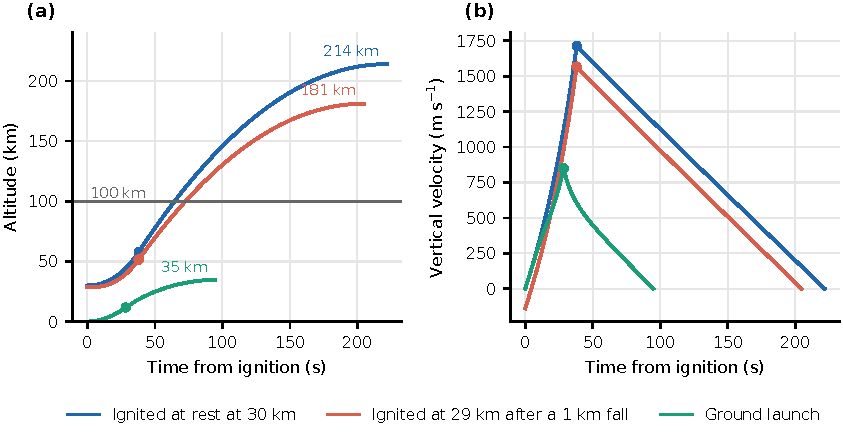
\includegraphics[width=\textwidth]{../paper/figures/fig_trajectory.pdf}
\caption{(a) Altitude and (b) vertical velocity of the baseline vehicle. Dots mark burnout.}
\label{fig:trajectory}
\end{figure}

\subsection{Decomposition of the gain}
\label{sec:decomp}

A balloon changes three things at once. The rocket starts higher, and gravity is slightly weaker (the head start). It flies through thinner air (drag). Its nozzle can have a larger area ratio and sees a lower back-pressure (nozzle). To separate them, the trajectory code keeps three altitude offsets: one for the position and gravity, one for the atmosphere used in the drag, and one for the atmosphere used in the nozzle selection and back-pressure. Each can be set to the ground or to the float altitude, which gives eight runs (Table~\ref{tab:runs}).

The effects are not additive. Removing drag is worth more when the nozzle is also better, because the rocket is then faster. We therefore attribute the gain by averaging the contribution of each effect over the six orders in which the three can be switched on, which is the Shapley value of cooperative game theory \cite{shapley1953}. The three contributions add up exactly to the total gain. The split depends on what is measured. In burnout velocity, the same eight runs give a gain of \R{dvbGain}$\ms$, of which drag supplies \R{dvbFDrag}\%, the nozzle \R{dvbFNozzle}\% and the head start \R{dvbFHead}\%; in the velocity budget of Table~\ref{tab:baseline}, the balloon launch saves \R{budLd}$\ms$ of drag loss and gains \R{budDvThr}$\ms$ of thrust $\Delta v$, and pays \R{budLg}$\ms$ more gravity loss. The apogee magnifies these terms unequally. Above burnout the rocket coasts almost without drag, so its apogee is close to $z_0+h_b+v_b^2/(2g)$, and a small change in burnout velocity changes the apogee by about $v_b/g$ times as much: \R{coastFactor}\,s for the balloon launch and \R{coastFactorGnd}\,s for the ground launch. A term that acts when the rocket is already fast is therefore worth more height, which is also why the order of switching matters. We report the apogee split because the apogee is what the mission asks for, with the velocity split alongside for comparison with velocity-budget treatments such as that of Sarigul-Klijn \emph{et al.} \cite{sarigul2005}. The average hides a real dependence on the order: for the baseline vehicle the drag contribution is \R{ordDragLo}--\R{ordDragHi}\% of the gain depending on when it is switched on, the nozzle contribution \R{ordNozzleLo}--\R{ordNozzleHi}\% and the head start \R{ordHeadLo}--\R{ordHeadHi}\%. The shares quoted below are the averages and should be read with these ranges. They also depend on the drag calibration of Sec.~\ref{M-sec:validation} of the paper. At the scale factor fitted to the Deacon ground firings (\R{deaCdFit}) the ground-launched apogee is \R{cdDeaGnd}\,km, the ratio \R{cdDeaRatio} and the shares \R{cdDeaFDrag}\% drag, \R{cdDeaFNozzle}\% nozzle and \R{cdDeaFHead}\% head start. At a scale factor of 2, which the rockoon apogees prefer, the ground-launched apogee falls to \R{cdTwoGnd}\,km, the ratio rises to \R{cdTwoRatio} and the shares become \R{cdTwoFDrag}/\R{cdTwoFNozzle}/\R{cdTwoFHead}\%. The balloon-launched apogee hardly moves (\R{cdDeaBal} and \R{cdTwoBal}\,km). The ordering of the three terms is the same in every case; the ratio is not a robust number, and the drag share is a lower bound if the rockoon calibration is right.

For the baseline at 30\,km, drag accounts for \R{decDrag}\,km of the \R{gainKm}\,km gain (\R{decFDrag}\%), the nozzle for \R{decNozzle}\,km (\R{decFNozzle}\%) and the head start for \R{decHead}\,km (\R{decFHead}\%). The head-start term is close to the float altitude itself, as expected. Table~\ref{tab:runs} shows the interaction directly: with drag alone removed the apogee is \R{runGBG}\,km, with the nozzle alone changed it is \R{runGGB}\,km, and with both it is \R{runGBB}\,km, more than the two separate gains added to the ground value.

Figure~\ref{fig:decomp} and Table~\ref{tab:decalt} show how the shares depend on float altitude. Drag is the largest term at every altitude, but its share falls from \R{decAltTenDrag}\% at 10\,km to \R{decFDrag}\% at 30\,km, as the head start grows. Most of the drag benefit is collected early, because the density has already fallen to about a third of its sea-level value at 10\,km.

\begin{figure}[!htb]
\centering
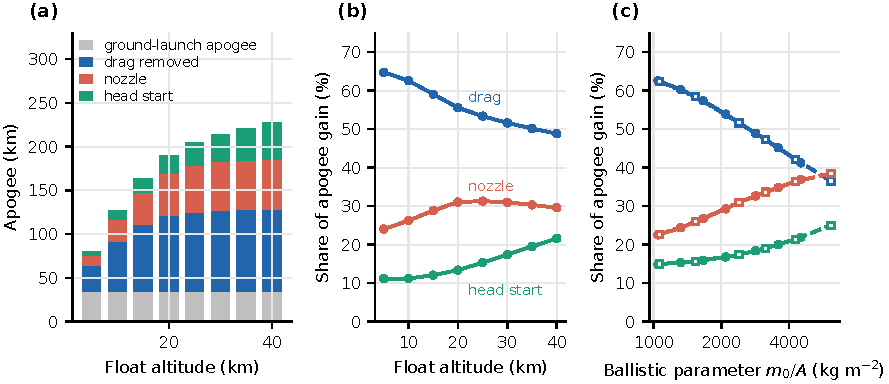
\includegraphics[width=\textwidth]{../paper/figures/fig_decomposition.pdf}
\caption{Decomposition of the apogee gain. (a) Baseline vehicle against float altitude: ground-launch apogee and the three contributions. (b) The same as shares of the gain. (c) Shares at a float altitude of 30\,km against the ballistic parameter. Colours as in (b). Filled symbols: gross mass varied from 25 to 2000\,kg at constant proportions. Open symbols: diameter of the 301\,kg vehicle varied from 0.25 to 0.60\,m.}
\label{fig:decomp}
\end{figure}

\begin{table}[!htb]
\centering
\caption{Baseline vehicle against float altitude: apogee from the ground and from the balloon, their ratio, and the shares of the gain.}
\label{tab:decalt}
\small
\begin{tabular}{ccccccc}
\toprule
Float altitude & \multicolumn{2}{c}{Apogee (km)} & Ratio & \multicolumn{3}{c}{Share of gain (\%)} \\
(km) & ground & balloon & & drag & nozzle & head start \\
\midrule
\tabin{tab_dec_alt.tex}
\bottomrule
\end{tabular}
\end{table}

\subsection{Dependence on vehicle size}

Table~\ref{tab:decmass} and Fig.~\ref{fig:decomp}(c) give the decomposition at 30\,km for vehicles from 25 to 2000\,kg. Small vehicles have a low ballistic parameter and lose most to drag on the ground. A 50\,kg vehicle reaches \R{decMassFiftyGnd}\,km from the ground and \R{decMassFiftyBal}\,km from the balloon, a factor of \R{decMassFiftyRatio}; \R{decMassFiftyDrag}\% of its gain is drag. A 2000\,kg vehicle of the same proportions reaches \R{decMassBigGnd}\,km from the ground and \R{decMassBigBal}\,km from the balloon, a factor of \R{decMassBigRatio}; drag is \R{decMassBigDrag}\% of the gain and the nozzle \R{decMassBigNozzle}\%. Varying the diameter at fixed mass moves the shares along nearly the same curve (open symbols in Fig.~\ref{fig:decomp}c), so within this family the ballistic parameter is the controlling quantity; Sec.~\ref{sec:collapse} tests how far that holds in general. Okninski \emph{et al.} \cite{okninski2016} found low-mass designs advantageous for their solid-propellant rockoon; the present result shows the same trend and gives its size.

The balloon-launched apogee itself depends little on size, between \R{decMassBigBal} and \R{decMassFiftyBal}\,km over this range. It is slightly higher for small vehicles. With the diameter scaled as $m_0^{1/3}$ and the thrust as $m_0$, the nozzle exit of a small vehicle can occupy a larger area per unit thrust, so the area limit allows a larger area ratio.

\begin{table}[!htb]
\centering
\caption{Vehicles of constant proportions ignited at 30\,km: diameter, ballistic parameter, apogees, ratio, and shares of the gain.}
\label{tab:decmass}
\small
\begin{tabular}{ccccccccc}
\toprule
$m_0$ & $d$ & $m_0/A$ & \multicolumn{2}{c}{Apogee (km)} & Ratio & \multicolumn{3}{c}{Share of gain (\%)} \\
(kg) & (m) & (kg\,m$^{-2}$) & ground & balloon & & drag & nozzle & head start \\
\midrule
\tabin{tab_dec_mass.tex}
\bottomrule
\end{tabular}
\end{table}

\subsection{What float altitude costs}
\label{sec:altcost}

Figure~\ref{fig:scaling}(a) shows the apogee against ignition altitude for five vehicle sizes, and Fig.~\ref{fig:scaling}(b) and Table~\ref{tab:altcost} set the apogee of the baseline against the balloon needed to carry it. Over the first 10\,km the apogee rises by \R{gndFirstTen}\,km for each kilometre of ignition altitude. Between 20 and 30\,km it rises by \R{altGainLow}\,km per kilometre, and between 30 and 40\,km by \R{altGainHigh}\,km per kilometre. The balloon volume meanwhile grows by a factor of \R{altVolRatioLow} from 20 to 30\,km and by a further factor of \R{altVolRatioHigh} from 30 to 40\,km, because the volume scales with the inverse of the air density and the envelope grows with it. At 20\,km the baseline already reaches \R{altApTwenty}\,km with a balloon of \R{altVTwenty}\,m$^3$; at 30\,km it reaches \R{balAp}\,km with \R{balV}\,m$^3$.

For the baseline at 30\,km the envelope weighs \R{balEnv}\,kg and the hydrogen \R{balH2}\,kg; with 10\% free lift for the ascent the launch inventory is about \R{balLaunchH2}\,kg. Helium would need \R{balHeVolPct}\% more volume and \R{balHeMassRatio} times the gas mass (\R{balHe}\,kg).

\begin{figure}[!htb]
\centering
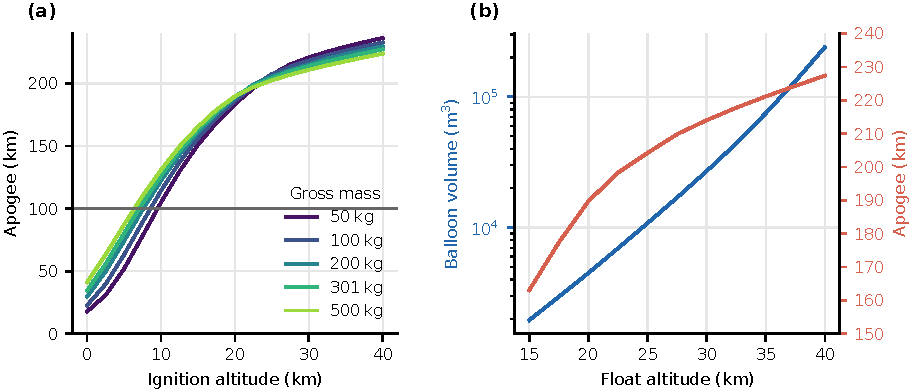
\includegraphics[width=\textwidth]{../paper/figures/fig_scaling.pdf}
\caption{(a) Apogee against ignition altitude for vehicles of constant proportions. (b) Balloon volume (hydrogen, 30\,kg gondola, $\sigma=30\,\mathrm{g\,m^{-2}}$) and apogee of the baseline vehicle against float altitude.}
\label{fig:scaling}
\end{figure}

\begin{table}[!htb]
\centering
\caption{Apogee of the baseline vehicle for the eight combinations of environments (float altitude 30\,km).}
\label{tab:runs}
\small
\begin{tabular}{cccc}
\toprule
Position and gravity & Drag & Nozzle & Apogee (km) \\
\midrule
\tabin{tab_runs.tex}
\bottomrule
\end{tabular}
\end{table}

\begin{table}[!htb]
\centering
\caption{Balloon for the baseline vehicle and a 30\,kg gondola, and the apogee reached, against float altitude.}
\label{tab:altcost}
\small
\begin{tabular}{ccccc}
\toprule
Float altitude & Volume & Envelope & Hydrogen at float & Apogee \\
(km) & (m$^3$) & (kg) & (kg) & (km) \\
\midrule
\tabin{tab_altcost.tex}
\bottomrule
\end{tabular}
\end{table}

\section{Test of the similarity hypothesis}
\label{sec:collapse}

To test H1 we drew \R{ensN} vehicles at random: gross mass 20--5000\,kg (log-uniform), fineness 8--20, bulk density 500--900$\kgm$, propellant fraction 0.40--0.60, thrust-to-weight ratio 2--6, float altitude 5--40\,km, drag scale factor 0.8--1.2, and one of four engines (the liquid engine at 1, 2 or 4\,MPa, or the generic solid motor of Sec.~\ref{M-sec:model} of the paper). Their $\Pi_D(0)$ ranges from \R{ensPiLo} to \R{ensPiHi}. Each vehicle was flown in the eight combinations of Sec.~\ref{sec:decomp}.

The drag loss of the ground launch collapses onto $\Pi_D(0)$ (Fig.~\ref{fig:collapse}a). As a fraction of the thrust $\Delta v$ it follows $\R{ldCoef}\,\Pi_D(0)^{\R{ldSlope}}$, a quadratic in $\ln\Pi_D(0)$ explains \R{fitLdOne} of its variance with a scatter of \R{fitLdOneSd}\% (\R{cvLd} out of sample), and the engine type makes no visible difference. The exponent is below the value of one suggested by Sec.~\ref{sec:groups} because a vehicle that loses more to drag is also slower, which limits the loss. Across the ensemble the ground launch loses \R{ensLdLo}--\R{ensLdHi}\% of its thrust $\Delta v$ to drag (5th--95th percentile), and the balloon launch a median of \R{ensLdBalMed}\%.

The shares of the gain do not collapse. $\Pi_D(0)$ alone explains \R{fitSdOne} of the variance of the drag share, and \R{fxThirtySd} when every vehicle is ignited at 30\,km, so that the float altitude cannot spread them. The rest of the scatter comes from the chamber pressure, the body size relative to the thrust, the thrust-to-weight ratio and the propellant fraction, none of which is in $\Pi_D$. A regression on six groups reaches $R^2=\R{fitSdFull}$ for the drag share, but it is a curve fit to a deterministic model, not a similarity law; it is given with its coefficients in Sec.~\ref{app:similarity}. H1 is therefore supported for the drag loss and rejected for the shares. Drag is the largest of the three contributions for \R{ensDragLargest}\% of the vehicles, and the drag share lies between \R{ensSdLo}\% and \R{ensSdHi}\% (5th--95th percentile).

\subsection{Regressions}
\label{app:similarity}


This subsection gives the regressions behind the statements above. Figure~\ref{fig:collapse} shows the ensemble and Table~\ref{tab:collapse} the variance explained by fits on one, three and six groups.

Unlike the drag loss, the shares of the gain do not collapse (Fig.~\ref{fig:collapse}b). $\Pi_D(0)$ alone explains \R{fitSdOne} of the variance of the drag share, \R{fitSnOne} for the nozzle share and \R{fitShOne} for the head start, and \R{fitROne} for the logarithm of the apogee ratio. Adding $\psi$ and $\xi$ helps a little. Adding $p_c/p_0$, $z_0/H$ and $\Pi_c$ as well brings the drag share to \R{fitSdFull} with a residual of \R{fitSdFullSd} percentage points (Fig.~\ref{fig:collapse}c), and the other shares to about the same. With the full set the solid-motor vehicles lie $\R{ensSolidOff}$ percentage points from the fit on average, so the engine type is captured by the pressure groups. The apogee ratio is the least well described, with a residual of \R{fitRFullSd}\% in the full fit.

The fits are not over-fitted: in five-fold cross-validation the out-of-sample $R^2$ is \R{cvLd} for the drag loss with $\Pi_D(0)$ alone, \R{cvSdOne} for the drag share with $\Pi_D(0)$ alone, and \R{cvSd} for the drag share with all six groups (residual \R{cvSdSd} percentage points).

The six-group fit is an empirical regression with eight coefficients fitted to the output of a deterministic model, so a high $R^2$ is expected and it is not a similarity law; its coefficients are in Table~\ref{tab:coef}. The one-group fit of the drag loss is $\ln(\Delta v_D/\Delta v)=\R{ldA}\,\R{ldB}\ln\Pi_D\,\R{ldC}(\ln\Pi_D)^2$.

Because the ensemble varies the float altitude, the shares could not collapse onto $\Pi_D(0)$ alone even in principle, so we flew the same \R{ensN} vehicles again with every one ignited at 30\,km. $\Pi_D(0)$ then explains \R{fxThirtySd} of the variance of the drag share (residual \R{fxThirtySdSd} points), \R{fxThirtySn} of the nozzle share and \R{fxThirtySh} of the head-start share; at 15\,km the values are \R{fxFifteenSd}, \R{fxFifteenSn} and \R{fxFifteenSh}. Fixing the float altitude therefore raises the drag share's $R^2$ from \R{fitSdOne} to \R{fxThirtySd}; the rest of the scatter comes from the engine and thrust groups.

\begin{figure}[!htb]
\centering
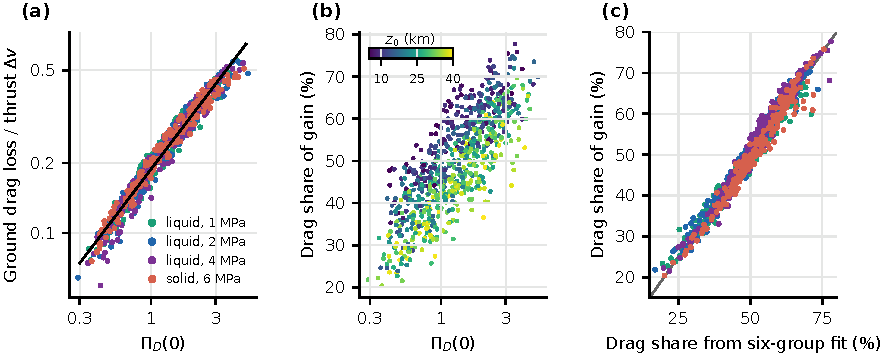
\includegraphics[width=\textwidth]{../paper/figures/fig_collapse.pdf}
\caption{Similarity test over \R{ensN} random vehicles. (a) Drag loss of the ground launch, as a fraction of the thrust $\Delta v$, against $\Pi_D(0)$, coloured by engine; the line is the power-law fit. (b) Drag share of the apogee gain against $\Pi_D(0)$, coloured by float altitude. (c) Drag share against the value given by the six-group fit.}
\label{fig:collapse}
\end{figure}

\begin{table}[!htb]
\centering
\caption{Variance explained ($R^2$) and residual standard deviation of least-squares fits over the ensemble, using $\Pi_D(0)$ alone (quadratic in $\ln\Pi_D$), with $\psi$ and $\xi$ added, and with $p_c/p_0$, $z_0/H$ and $\Pi_c$ added as well. Residuals are in per cent for the logarithmic quantities and in percentage points (pp) for the shares.}
\label{tab:collapse}
\small
\begin{tabular}{lcccccc}
\toprule
 & \multicolumn{2}{c}{$\Pi_D(0)$} & \multicolumn{2}{c}{$+\,\psi,\ \xi$} & \multicolumn{2}{c}{$+\,p_c/p_0,\ z_0/H,\ \Pi_c$} \\
Quantity & $R^2$ & resid. & $R^2$ & resid. & $R^2$ & resid. \\
\midrule
\tabin{tab_collapse.tex}
\bottomrule
\end{tabular}
\end{table}

\begin{table}[!htb]
\centering
\caption{Coefficients of the six-group least-squares fits of Sec.~\ref{sec:collapse}. Each quantity is the sum of the listed terms times the coefficients. The fits hold only inside the sampled ranges: $\Pi_D(0)$ from \R{ensPiLo} to \R{ensPiHi}, $\psi$ from \R{rngPsiLo} to \R{rngPsiHi}, and $\Pi_c$ from \R{rngPicLo} to \R{rngPicHi}, with the other ranges as in Sec.~\ref{sec:collapse}.}
\label{tab:coef}
\small
\begin{tabular}{lcccc}
\toprule
Term & $S_D$ & $S_N$ & $S_H$ & $\ln R$ \\
\midrule
\tabin{tab_coef.tex}
\bottomrule
\end{tabular}
\end{table}

\section{Robustness and uncertainty}
\label{sec:robustsec}

\subsection{Design of the comparison}
\label{sec:robust}

Three choices in the comparison above could favour the balloon, and a fourth is uncertain. We test all four.

First, the ground-launched vehicle has so far been the balloon vehicle with a different nozzle. A vehicle designed for ground launch would be slimmer. Taking the baseline body to have a length-to-diameter ratio of 10, we let each vehicle choose its own ratio between 10 and 20 at constant volume, and its own thrust-to-weight ratio up to \R{twMax} (a burnout acceleration of 15\,$g$). The ground-launched vehicle then prefers the slimmest body (\R{optGndD}\,m) and a thrust-to-weight ratio of \R{optGndTw}, and reaches \R{optGndAp}\,km. The balloon-launched vehicle keeps the 0.40\,m body, whose larger base allows a larger nozzle, takes a thrust-to-weight ratio of \R{optBalTw}, and reaches \R{optBalAp}\,km. With each vehicle designed for its own launch the ratio is \R{optRatio} instead of \R{gainRatio}, and the gain is \R{optGain}\,km instead of \R{gainKm}\,km. If both vehicles use the slim \R{slimD}\,m body, the apogees are \R{slimGnd} and \R{slimBal}\,km and the shares are \R{slimFDrag}\% drag, \R{slimFNozzle}\% nozzle and \R{slimFHead}\% head start. Drag remains the largest term, but by a smaller margin.

Second, the rule that the ground nozzle may not over-expand is stricter than practice: sea-level engines commonly run with an exit pressure below ambient, down to a separation limit of roughly 0.4 of ambient \cite{sutton2017}. We therefore let the exit pressure of the ground nozzle fall to between 1.0 and 0.4 of ambient in steps of 0.1. The ground-launched apogee is highest at \R{sepBest} of ambient (area ratio \R{sepEps}): \R{sepGnd}\,km against \R{gndApOne}\,km, a ratio of \R{sepRatio}, with shares of \R{sepFDrag}\% drag, \R{sepFNozzle}\% nozzle and \R{sepFHead}\% head start. At the limit of 0.4 (area ratio \R{sepLimEps}) the apogee is lower, \R{sepLimGnd}\,km, because this vehicle burns out low in the atmosphere and the thrust lost near the ground outweighs what is recovered later. With both freedoms together (its own body and thrust, and any over-expansion down to 0.4) the ground-launched vehicle reaches \R{sepOptGnd}\,km and the ratio is \R{sepOptRatio}. In this model the nozzle rule changes the ratio by about 0.1 and the nozzle share by about one point. The attribution does not count the mass and length of the larger nozzle at altitude, which would reduce the nozzle term; the closures of Sec.~\ref{M-sec:saving} of the paper count its mass.

Third, the nozzle term depends on the chamber pressure, because a higher pressure allows a larger area ratio on the ground. Table~\ref{tab:pc} repeats the calculation at 1, 2 and 4\,MPa. The nozzle share falls from \R{pcOneFNozzle}\% at 1\,MPa to \R{pcFourFNozzle}\% at 4\,MPa and the apogee ratio from \R{pcOneRatio} to \R{pcFourRatio}. The ordering of the three terms does not change.

Fourth, the drag curve of the baseline vehicle is assumed. With the curve computed by component build-up (Sec.~\ref{M-sec:traj} of the paper) the ground-launched apogee is \R{buGnd}\,km ($\R{buGndChange}$\%), the balloon-launched apogee is \R{buBal}\,km, and the shares are \R{buFDrag}\% drag, \R{buFNozzle}\% nozzle and \R{buFHead}\% head start. As a more severe test of the shape we also replaced it by the tabulated curve of a real sounding rocket, the booster-plus-dart configuration of the Super Loki \cite{bollermann1968}, which has a much higher transonic and supersonic drag coefficient (0.93 between Mach 0.8 and 1.4). The ground-launched apogee changes by $\R{acGndChange}$\% to \R{acGnd}\,km and the balloon-launched one by $\R{acBalChange}$\% to \R{acBal}\,km. The shares become \R{acFDrag}\% drag, \R{acFNozzle}\% nozzle and \R{acFHead}\% head start. The balloon-launched result does not depend on the drag curve; the ground-launched one, and with it the apogee ratio (\R{acRatio}), does. The build-up result shows that for a conventional slender geometry the change is modest.

\begin{table}[!htb]
\centering
\caption{Baseline vehicle at three chamber pressures ($\mathrm{O/F}=2.4$, float altitude 30\,km): selected area ratios and specific impulse at ignition on the ground (g) and at 30\,km (b), apogees, ratio, and shares of the gain.}
\label{tab:pc}
\small
\begin{tabular}{ccccccccccc}
\toprule
$p_c$ & \multicolumn{2}{c}{$\varepsilon$} & \multicolumn{2}{c}{$\Isp$ (s)} & \multicolumn{2}{c}{Apogee (km)} & Ratio & \multicolumn{3}{c}{Share of gain (\%)} \\
(MPa) & g & b & g & b & ground & balloon & & drag & nozzle & head \\
\midrule
\tabin{tab_pc.tex}
\bottomrule
\end{tabular}
\end{table}

\subsection{Non-vertical ignition}
\label{sec:tilt}

A rocket under a balloon will not be exactly vertical at ignition. We repeated the baseline case with a planar point-mass model for ignition at an angle to the vertical (Table~\ref{tab:tilt}). Two idealisations bracket the behaviour. In the first the thrust keeps its initial direction, as for a spin-stabilised or attitude-held vehicle; this is the relevant case at 30\,km, where there is no air to turn the body. In the second the thrust follows the velocity after 10\,m of guided travel (a gravity turn), as for an aerodynamically stable vehicle leaving a rail on the ground. Wind is not modelled; a balloon drifts with the wind, so the relative wind at ignition is small, as Okninski \emph{et al.} \cite{okninski2016} also note, whereas a ground launch meets the full wind profile.

With the attitude held, a tilt of 5$^{\circ}$ costs the balloon launch \R{tiltFixedLossFive}\% of its apogee and a tilt of 10$^{\circ}$ costs \R{tiltFixedLossTen}\%; at 20$^{\circ}$ the loss is \R{tiltFixedLossTwenty}\% and the vehicle travels \R{tiltRangeTwenty}\,km downrange. If instead the vehicle were allowed to gravity-turn from rest at 30\,km the loss would be far larger (\R{tiltTurnLossTen}\% at 10$^{\circ}$), because the turn is fastest when the speed is lowest. A balloon-launched vehicle therefore needs its attitude held through the first seconds of the burn, which is the problem that the suspended-launcher experiments address \cite{shoyama2021,shoyama2026}. The ground launch with a gravity turn loses \R{tiltGndLossTen}\% at 10$^{\circ}$. The conclusion that the balloon launch reaches several times the ground-launch apogee holds at every tilt examined, provided the attitude is held.

\begin{table}[!htb]
\centering
\caption{Baseline vehicle ignited at an angle from the vertical (planar model): apogee and downrange distance at apogee from 30\,km with the thrust direction held and with a gravity turn, ground-launch apogee with a gravity turn, and the ratio of the first to the last.}
\label{tab:tilt}
\small
\begin{tabular}{ccccccc}
\toprule
Tilt & \multicolumn{2}{c}{30\,km, attitude held} & \multicolumn{2}{c}{30\,km, gravity turn} & Ground, gravity turn & Ratio \\
(deg) & apogee (km) & range (km) & apogee (km) & range (km) & apogee (km) & \\
\midrule
\tabin{tab_tilt.tex}
\bottomrule
\end{tabular}
\end{table}

\subsection{Which results are robust}

Table~\ref{tab:robust} separates the findings that survived every variation we tried from those that depend on the idealised set-up.

\begin{table}[!htb]
\centering
\caption{Sensitivity of the main findings to the assumptions varied in this paper.}
\label{tab:robust}
\footnotesize
\begin{tabular}{@{}>{\raggedright\arraybackslash}p{5.2cm}>{\raggedright\arraybackslash}p{5.6cm}>{\raggedright\arraybackslash}p{3.4cm}@{}}
\toprule
Finding & Varied & Outcome \\
\midrule
Balloon-launched apogee is insensitive to drag & Drag scale 0.5--2; computed build-up curve; Super Loki drag table; Sobol analysis & Robust (changes below 1\%) \\
Ground drag loss scales with $\Pi_D(0)$ & 800 vehicles, four engines; cross-validation & Robust ($R^2=\R{cvLd}$ out of sample) \\
Drag is the largest share of the gain & Float altitude, size, chamber pressure, body shape, drag table, Monte Carlo & Holds in every single-vehicle case except the slimmest body (0.25\,m), where the nozzle share is one point larger; \R{ensDragLargest}\% of the ensemble \\
Mass-optimal float altitude near 20\,km (location) & 14 families, three target apogees, envelope density and a law fitted to published balloons, gondola fraction, load-scaled envelope, thermal jacket, nozzle mass, comparators designed for their own launch, cost weighting, Monte Carlo over the penalties & Robust: nominal \R{zsLo}--\R{zsHi}\,km, \R{mcsZLo}--\R{mcsZHi}\,km over the Monte Carlo; explained by Eq.~(\ref{M-eq:rule}) of the paper \\
Saving relative to ground launch & Comparators designed for ground launch, two-stage and solid comparators, nozzle mass, gondola, envelope law, cost weighting, Monte Carlo & Not robust: probability of a saving at least \R{mcsSsPLo}\% (steel tanks), \R{mcsAlPLo}--\R{mcsAlPHi}\% (aluminium) \\
Thermochemistry & NASA CEA run directly, shifting and frozen, O/F 1.6--3.6 & Within \R{ceaMaxDiff}\% \\
Trajectory integration & RocketPy, three and six degrees of freedom, baseline from the ground and from 30\,km & Apogees within \R{rpMaxDiff}\% \\
Drag-coefficient uncertainty vanishes once $\Pi_D(z_0)$ is below about 0.2 & Sobol indices with bootstrap intervals; four vehicles & Robust over $\Pi_D(0)=0.8$--3.7 \\
Apogee ratio of 6.2 for the baseline & Drag scale \R{deaCdFit} and 2 (\R{cdDeaRatio}, \R{cdTwoRatio}); fair comparator (\R{optRatio}); best over-expanded ground nozzle (\R{sepRatio}); build-up drag (\R{buRatio}); Super Loki drag table (\R{acRatio}); tilt & Depends on the set-up \\
Exact shares 52/31/17\% & Switching order, drag scale, chamber pressure, nozzle rule, body shape, drag table & Vary by about ten points; drag share \R{cdTwoFDrag}\% at a drag scale of 2 \\
Absolute apogees & Efficiency, dry mass, tilt, validation offset of about 6\% & Model outputs only \\
\bottomrule
\end{tabular}
\end{table}

\subsection{Monte Carlo and variance-based sensitivity}
\label{sec:mc}

To see how firm these results are we drew \R{mcN} samples of five inputs for the baseline vehicle and flew each one from the balloon and from the ground. The inputs and their ranges are: drag scale factor, uniform on 0.8--1.2 (Sec.~\ref{M-sec:traj} of the paper); efficiency $\eta$, uniform on 0.85--0.95; thrust-to-weight ratio, uniform on 3--5; dry mass, normal with a standard deviation of 5\%; and float altitude, uniform on 28--32\,km. Apart from the drag range these are our assumptions.

The balloon-launched apogee has a median of \R{mcBalMed}\,km and a 5th--95th percentile range of \R{mcBalLo}--\R{mcBalHi}\,km (Fig.~\ref{fig:mc}a). None of the samples falls below 100\,km. The median lies below the baseline value of \R{balAp}\,km because the sampled efficiency range is centred on 0.90, not on the nominal 0.92. The ground-launched apogee is \R{mcGndMed}\,km (\R{mcGndLo}--\R{mcGndHi}\,km), and the ratio of the two is \R{mcRatioMed} (\R{mcRatioLo}--\R{mcRatioHi}). The coefficient of variation is \R{mcBalCv}\% from the balloon and \R{mcGndCv}\% from the ground.

The two cases are uncertain for different reasons. The rank correlation of the ground-launched apogee with the drag scale factor is $\R{rhoGndCd}$; for the balloon-launched apogee it is $\R{rhoBalCd}$. The balloon-launched apogee is controlled instead by the dry mass ($\R{rhoBalDry}$) and the efficiency ($\R{rhoBalEta}$). A balloon launch therefore removes the quantity that is hardest to predict without wind-tunnel or flight data.

To follow this with altitude we computed variance-based (Sobol) sensitivity indices, using the estimators of Jansen \cite{jansen1999,saltelli2010}, of the apogee to the first four inputs at eleven ignition altitudes, with \R{sobN} base samples each (Fig.~\ref{fig:sobol}). The total-effect index of the drag scale factor is \R{sobCdZero} at the ground (95\% bootstrap interval \R{sobCdZeroLo}--\R{sobCdZeroHi}), \R{sobCdFive} at 5\,km and \R{sobCdTen} at 10\,km (\R{sobCdTenLo}--\R{sobCdTenHi}), and is below 0.01 from 15\,km upward, where $\Pi_D(z_0)\approx\R{sobPiFifteen}$. For one vehicle, plotting against $\Pi_D(z_0)$ only relabels the altitude axis, so to test H3 we repeated the calculation for four vehicles with $\Pi_D(0)$ from \R{h3PiZeroLo} to \R{h3PiZeroHi}: 30, 301 and 3000\,kg with the baseline proportions, and a 301\,kg vehicle twice as slender, each with \R{h3NS} base samples (Fig.~\ref{fig:sobol}b,c). The index falls below 0.01 at altitudes from \R{h3ZLo} to \R{h3ZHi}\,km but at nearly the same $\Pi_D(z_0)$, \R{h3PiLo}--\R{h3PiHi}. A cubic in $\ln\Pi_D(z_0)$ explains \R{h3RPi} of the variance of the pooled index, against \R{h3RZ} for a cubic in altitude. H3 holds over this range: the drag coefficient stops mattering once $\Pi_D(z_0)$ falls to about 0.1--0.2, wherever that happens. Above 15\,km the apogee variance is shared between the dry mass (\R{sobDryThirty} at 30\,km) and the efficiency (\R{sobEtaThirty}).

The decomposition is stable. Over \R{mcNshap} samples the drag share is \R{mcFDragMed}\% (\R{mcFDragLo}--\R{mcFDragHi}\%), the nozzle share \R{mcFNozzleMed}\% (\R{mcFNozzleLo}--\R{mcFNozzleHi}\%) and the head-start share \R{mcFHeadMed}\% (\R{mcFHeadLo}--\R{mcFHeadHi}\%), and drag is the largest term in every sample (Fig.~\ref{fig:mc}b).

One-at-a-time changes give the same picture. From the balloon, thrust-to-weight ratios of 2 and 8 give \R{sTwLo} and \R{sTwHi}\,km, and halving or doubling the drag coefficient gives \R{sCdLo} and \R{sCdHi}\,km. From the ground, drag scale factors of 0.8 and 1.2 give \R{sGndCdLo} and \R{sGndCdHi}\,km, and bodies of 0.35 and 0.30\,m give \R{sGndD35} and \R{sGndD30}\,km.

\begin{figure}[!htb]
\centering
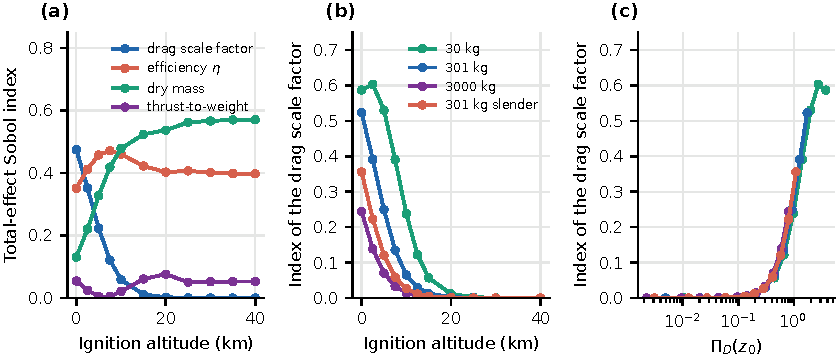
\includegraphics[width=\textwidth]{../paper/figures/fig_sobol.pdf}
\caption{Total-effect Sobol indices of the apogee. (a) Baseline vehicle, four inputs, against ignition altitude. (b) Index of the drag scale factor for four vehicles against ignition altitude. (c) The same against $\Pi_D(z_0)$.}
\label{fig:sobol}
\end{figure}

\begin{figure}[!htb]
\centering
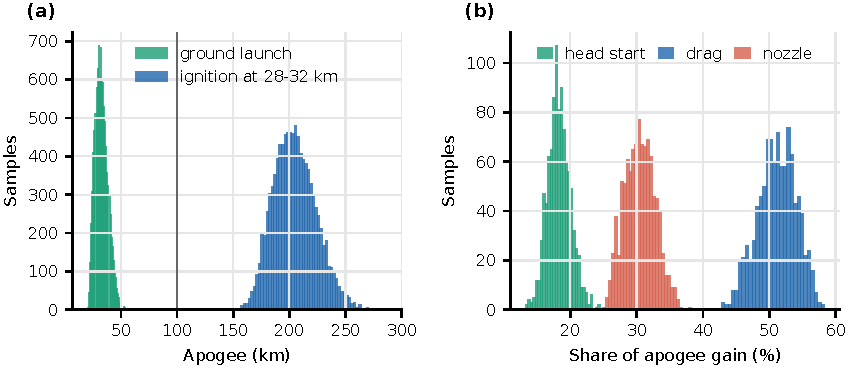
\includegraphics[width=\textwidth]{../paper/figures/fig_montecarlo.pdf}
\caption{Monte Carlo results for the baseline vehicle. (a) Apogee from the ground and from the balloon (\R{mcN} samples). (b) Shares of the apogee gain (\R{mcNshap} samples).}
\label{fig:mc}
\end{figure}

\subsection{Error budget}

Four kinds of error enter the results, and they differ greatly in size. (i) \emph{Numerical}: the integration error is below 0.1\,m in apogee (Sec.~\ref{M-sec:validation} of the paper), and the planar model at zero tilt reproduces the vertical model to within $10^{-4}$. (ii) \emph{Sampling}: with \R{mcN} samples the bootstrap standard error of the median apogee is \R{mcBalMedSe}\,km from the balloon and \R{mcGndMedSe}\,km from the ground; the Sobol index of the drag coefficient at the ground has a 95\% interval of \R{sobCdZeroLo}--\R{sobCdZeroHi}; the regression residuals are unchanged out of sample. (iii) \emph{Parametric}: the 5th--95th percentile range of the balloon-launched apogee is \R{mcBalLo}--\R{mcBalHi}\,km, about $\pm$15\%, driven by dry mass and engine efficiency. (iv) \emph{Model form}: against the flights and published trajectories available to us the model is high by $\R{deaErrMean}$\% in burnout velocity for the Deacon and by about 6\% in apogee for the Super Loki, and it is within about 10\% r.m.s. of nine rockoon apogees once a mass is fitted; NASA CEA and RocketPy reproduce its thermochemistry and its integration to \R{ceaMaxDiff}\% and \R{rpMaxDiff}\%. It omits attitude dynamics, wind and real-gas and structural effects. The model-form and parametric errors dominate. The numerical and sampling errors are negligible beside them, so further gains in accuracy must come from better physics and better input data, not from finer computation.

\section{Propellant performance against mixture ratio}
\label{app:thermo}

Figure~\ref{fig:appendix} shows the ideal vacuum specific impulse at an area ratio of 36.4 and the chamber temperature at 2.0\,MPa against mixture ratio, from our calculation and from NASA CEA run directly \cite{cea2026}. The specific impulse peaks at \R{ispShiftPeak}\,s near $\mathrm{O/F}=\R{ofShiftPeak}$ for shifting equilibrium and at \R{ispFrozenPeak}\,s near $\mathrm{O/F}=\R{ofFrozenPeak}$ for a composition frozen at the chamber state. At the design point, $\mathrm{O/F}=2.4$, the values are \R{ispShift}\,s and \R{ispFrozen}\,s, and the delivered value used in the paper is \R{ispDel}\,s (\R{ispDelLo}--\R{ispDelHi}\,s for $\eta=0.85$--0.95). For 68\,atm expanded to 1\,atm the frozen value at $\mathrm{O/F}=2.1$ is \R{bmFrozen}\,s. The calculation is gas-phase only and is not used below $\mathrm{O/F}=0.8$ except for the single point quoted in the supplementary audit.

\begin{figure}[!htb]
\centering
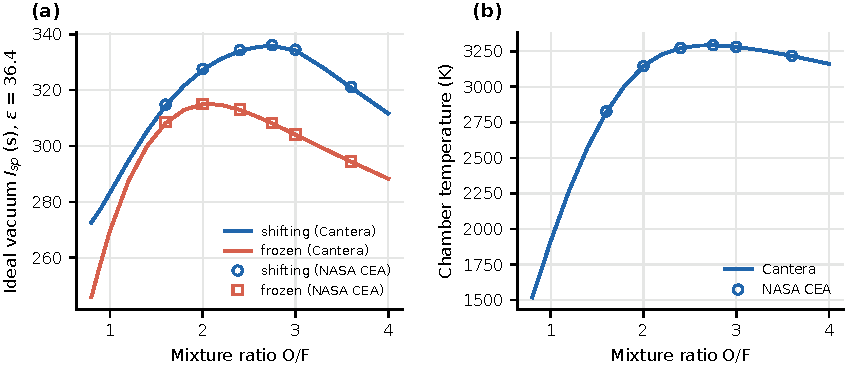
\includegraphics[width=\textwidth]{../paper/figures/fig_appendix.pdf}
\caption{(a) Ideal vacuum specific impulse of UDMH/N$_2$O$_4$ at 2.0\,MPa and an area ratio of 36.4, from our Cantera calculation (lines) and from NASA CEA run directly (symbols). (b) Chamber temperature.}
\label{fig:appendix}
\end{figure}

\begin{thebibliography}{99}

\bibitem{allen1958} H.\,J. Allen and A.\,J. Eggers, Jr., \emph{A Study of the Motion and Aerodynamic Heating of Ballistic Missiles Entering the Earth's Atmosphere at High Supersonic Speeds}, NACA Report 1381 (National Advisory Committee for Aeronautics, Washington, DC, 1958).

\bibitem{shapley1953} L.\,S. Shapley, ``A value for $n$-person games,'' in \emph{Contributions to the Theory of Games II}, edited by H.\,W. Kuhn and A.\,W. Tucker, Annals of Mathematics Studies \textbf{28} (Princeton University Press, Princeton, NJ, 1953), pp.~307--317.

\bibitem{sarigul2005} N. Sarigul-Klijn, M. Sarigul-Klijn, and C. Noel, ``Air-launching Earth to orbit: effects of launch conditions and vehicle aerodynamics,'' J. Spacecr. Rockets \textbf{42}, 569--575 (2005), doi:10.2514/1.8634.

\bibitem{okninski2016} A. Okninski, D. Sors Raurell, and A. Rodriguez Mitre, ``Feasibility of a low-cost sounding rockoon platform,'' Acta Astronaut. \textbf{127}, 335--344 (2016), doi:10.1016/j.actaastro.2016.06.010.

\bibitem{sutton2017} G.\,P. Sutton and O. Biblarz, \emph{Rocket Propulsion Elements}, 9th ed. (Wiley, Hoboken, NJ, 2017).

\bibitem{bollermann1968} B. Bollermann and R.\,L. Walker, \emph{Super Loki Dart Meteorological Rocket System}, NASA CR-61238 (Space Data Corporation, Phoenix, AZ, 30 June 1968), \url{https://ntrs.nasa.gov/citations/19680026183}.

\bibitem{shoyama2021} T. Shoyama, A. Banno, Y. Furuta, N. Kurata, D. Ode, Y. Wada, and T. Matsui, ``Air-launch experiment using suspended rail launcher for rockoon,'' Aerospace \textbf{8}, 289 (2021), doi:10.3390/aerospace8100289.

\bibitem{shoyama2026} T. Shoyama, Y. Wada, and S. Oda, ``Rockoon launch experiment with azimuth angle control,'' Aerospace \textbf{13}, 709 (2026), doi:10.3390/aerospace13080709.

\bibitem{jansen1999} M.\,J.\,W. Jansen, ``Analysis of variance designs for model output,'' Comput. Phys. Commun. \textbf{117}, 35--43 (1999), doi:10.1016/S0010-4655(98)00154-4.

\bibitem{saltelli2010} A. Saltelli, P. Annoni, I. Azzini, F. Campolongo, M. Ratto, and S. Tarantola, ``Variance based sensitivity analysis of model output. Design and estimator for the total sensitivity index,'' Comput. Phys. Commun. \textbf{181}, 259--270 (2010).

\bibitem{cea2026} National Aeronautics and Space Administration, \emph{CEA: Chemical Equilibrium with Applications}, version 3.3.4, Python package, \url{https://nasa.github.io/cea} (accessed 18 November 2026).

\end{thebibliography}

\end{document}
